\documentclass[a4 paper, 15pt]{article}
% Set target color model to RGB
\usepackage[inner=2.0cm,outer=2.0cm,top=2.5cm,bottom=2.5cm]{geometry}
\usepackage{setspace}
\usepackage[rgb]{xcolor}
\usepackage{verbatim}
\usepackage{subcaption, float}
\usepackage{amsgen,amsmath,amstext,amsbsy,amsopn,tikz,amssymb,tkz-linknodes}
\usepackage{fancyhdr, graphicx}
\usepackage[colorlinks=true, urlcolor=blue,  linkcolor=blue, citecolor=blue]{hyperref}
\usepackage[colorinlistoftodos]{todonotes}
\usepackage{rotating}
%\usetikzlibrary{through,backgrounds}
\hypersetup{%
pdfauthor={Ashudeep Singh},%
pdftitle={Homework},%
pdfkeywords={Tikz,latex,bootstrap,uncertaintes},%
pdfcreator={PDFLaTeX},%
pdfproducer={PDFLaTeX},%
}
%\usetikzlibrary{shadows}
\usepackage{booktabs}
\newcommand{\ra}[1]{\renewcommand{\arraystretch}{#1}}
\newcommand{\norm}[1]{\left\lVert#1\right\rVert}

\newtheorem{thm}{Theorem}[section]
\newtheorem{prop}[thm]{Proposition}
\newtheorem{lem}[thm]{Lemma}
\newtheorem{cor}[thm]{Corollary}
\newtheorem{defn}[thm]{Definition}
\newtheorem{rem}[thm]{Remark}
\numberwithin{equation}{section}

\newcommand{\homework}[6]{
   \pagestyle{myheadings}
   \thispagestyle{plain}
   \newpage
   \setcounter{page}{1}
   \noindent
   \begin{center}
   \framebox{
      \vbox{\vspace{2mm}
    \hbox to 6.28in { {\bf CS 6780:~Advanced Machine Learning \hfill {\small (#2)}} }
       \vspace{6mm}
       \hbox to 6.28in { {\Large \hfill #1  \hfill} }
       \vspace{6mm}
       \hbox to 6.28in { {\it Instructor: {\rm #3} \hfill Name: {\rm #5}, Netid: {\rm #6}} }
       %\hbox to 6.28in { {\it TA: #4  \hfill #6}}
      \vspace{2mm}}
   }
   \end{center}
   \markboth{#5 -- #1}{#5 -- #1}
   \vspace*{4mm}
}
\newcommand{\problem}[1]{~\\\fbox{\textbf{Problem #1}}\newline\newline}
\newcommand{\subproblem}[1]{~\newline\textbf{(#1)}}
\newcommand{\D}{\mathcal{D}}
\newcommand{\Hy}{\mathcal{H}}
\newcommand{\VS}{\textrm{VS}}
\newcommand{\solution}{~\newline\textbf{\textit{(Solution)}} }


\begin{document}
\homework{Submission Assignment \#2}{Submitted on: 3/6/2019}{Thorsten Joachims}{}{Molly Ingram, Julien Neves}{msi34, jmn252}

\problem{1}
\subproblem{a}

Figure \ref{fig:1} shows one possible labeling and solution where we have one $-$ and three $+$. To get every possible iteration of one $-$ and three $+$, we simply need to rotate the points and the ellipse by 90$^\circ$, 180$^\circ$ and 270$^\circ$.
\begin{figure}[H]
  \centering
  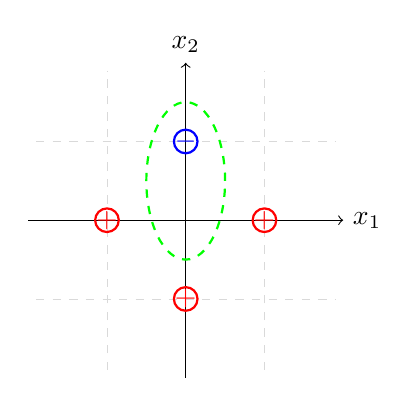
\begin{tikzpicture}
  \draw[help lines, color=gray!30, dashed] (-1.9,-1.9) grid (1.9,1.9);
  \draw[->] (-2,0)--(2,0) node[right]{$x_1$};
  \draw[->] (0,-2)--(0,2) node[above]{$x_2$};
  \draw [blue, thick] (0,1) circle (.15cm) node[]{$-$};
  \draw [red, thick] (0,-1) circle (.15cm) node[]{$+$};
  \draw [red, thick] (1,0) circle (.15cm) node[]{$+$};
  \draw [red, thick] (-1,0) circle (.15cm) node[]{$+$};
  \draw [green, thick, dashed](0,0.5) ellipse (.5cm and 1cm);
  \end{tikzpicture}
  \caption{One $-$ and three $+$}
  \label{fig:1}
\end{figure}

Figure \ref{fig:2} shows two possible labeling and solutions where we have two $-$ and two $+$. To get every possible iteration, we simply need to rotate the first figure by 180$^\circ$ and flip the second figure along the both the $x_1$ and $x_2$ axes.
\begin{figure}[H]
  \centering
\begin{subfigure}[b]{0.3\textwidth}
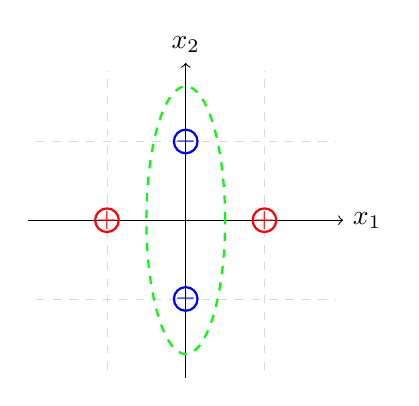
\begin{tikzpicture}
\draw[help lines, color=gray!30, dashed] (-1.9,-1.9) grid (1.9,1.9);
\draw[->] (-2,0)--(2,0) node[right]{$x_1$};
\draw[->] (0,-2)--(0,2) node[above]{$x_2$};
\draw [blue, thick] (0,1) circle (.15cm) node[]{$-$};
\draw [blue, thick] (0,-1) circle (.15cm) node[]{$-$};
\draw [red, thick] (1,0) circle (.15cm) node[]{$+$};
\draw [red, thick] (-1,0) circle (.15cm) node[]{$+$};
\draw [green, thick, dashed](0,0) ellipse (.5cm and 1.7cm);
\end{tikzpicture}
\end{subfigure}
\begin{subfigure}[b]{0.3\textwidth}
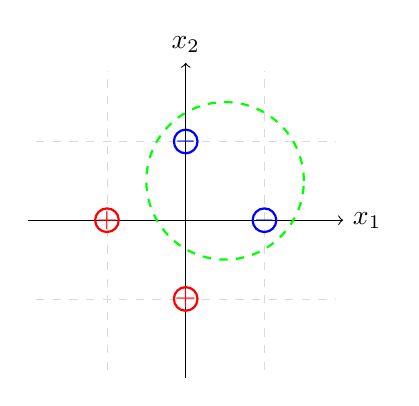
\begin{tikzpicture}
\draw[help lines, color=gray!30, dashed] (-1.9,-1.9) grid (1.9,1.9);
\draw[->] (-2,0)--(2,0) node[right]{$x_1$};
\draw[->] (0,-2)--(0,2) node[above]{$x_2$};
\draw [blue, thick] (0,1) circle (.15cm) node[]{$-$};
\draw [red, thick] (0,-1) circle (.15cm) node[]{$+$};
\draw [blue, thick] (1,0) circle (.15cm) node[]{$-$};
\draw [red, thick] (-1,0) circle (.15cm) node[]{$+$};
\draw [green, thick, dashed](0.5,0.5) ellipse (1cm and 1cm);
\end{tikzpicture}
\end{subfigure}

  \caption{Two $-$ and two $+$}
\label{fig:2}
\end{figure}


Figure \ref{fig:3} shows one possible labeling and solution where we have three $-$ and one $+$. To get every possible iteration of three $-$ and one $+$, we simply need to rotate the points and the ellipse by 90$^\circ$, 180$^\circ$ and 270$^\circ$.
\begin{figure}[H]
  \centering
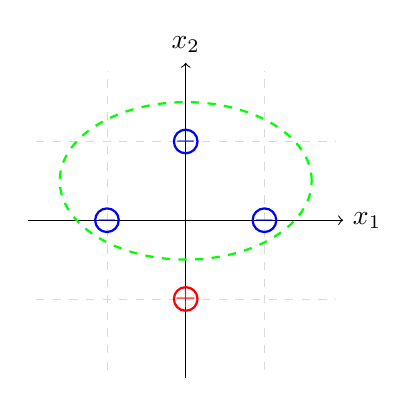
\begin{tikzpicture}
\draw[help lines, color=gray!30, dashed] (-1.9,-1.9) grid (1.9,1.9);
\draw[->] (-2,0)--(2,0) node[right]{$x_1$};
\draw[->] (0,-2)--(0,2) node[above]{$x_2$};
\draw [blue, thick] (0,1) circle (.15cm) node[]{$-$};
\draw [red, thick] (0,-1) circle (.15cm) node[]{$+$};
\draw [blue, thick] (1,0) circle (.15cm) node[]{$-$};
\draw [blue, thick] (-1,0) circle (.15cm) node[]{$-$};
\draw [green, thick, dashed](0,.5) ellipse (1.6cm and 1cm);
\end{tikzpicture}
  \caption{Three $-$ and one $+$}
\label{fig:3}
\end{figure}

Figure \ref{fig:4} shows the case where we have four $-$ or four $+$.
\begin{figure}[H]
  \centering
  \begin{subfigure}[b]{0.3\textwidth}
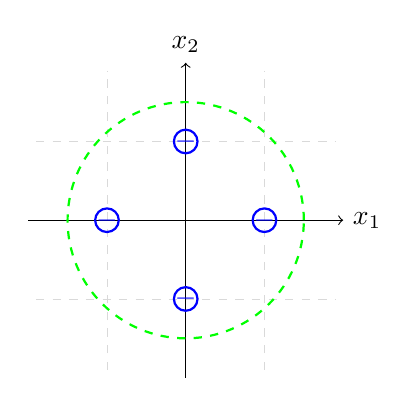
\begin{tikzpicture}
\draw[help lines, color=gray!30, dashed] (-1.9,-1.9) grid (1.9,1.9);
\draw[->] (-2,0)--(2,0) node[right]{$x_1$};
\draw[->] (0,-2)--(0,2) node[above]{$x_2$};
\draw [blue, thick] (0,1) circle (.15cm) node[]{$-$};
\draw [blue, thick] (0,-1) circle (.15cm) node[]{$-$};
\draw [blue, thick] (1,0) circle (.15cm) node[]{$-$};
\draw [blue, thick] (-1,0) circle (.15cm) node[]{$-$};
\draw [green, thick, dashed](0,0) ellipse (1.5cm and 1.5cm);
\end{tikzpicture}
\end{subfigure}
\begin{subfigure}[b]{0.3\textwidth}
  \begin{tikzpicture}
  \draw[help lines, color=gray!30, dashed] (-1.9,-1.9) grid (1.9,1.9);
  \draw[->] (-2,0)--(2,0) node[right]{$x_1$};
  \draw[->] (0,-2)--(0,2) node[above]{$x_2$};
  \draw [red, thick] (0,1) circle (.15cm) node[]{$+$};
  \draw [red, thick] (0,-1) circle (.15cm) node[]{$+$};
  \draw [red, thick] (1,0) circle (.15cm) node[]{$+$};
  \draw [red, thick] (-1,0) circle (.15cm) node[]{$+$};
  \draw [green, thick, dashed](0,0) ellipse (.5cm and .5cm);
  \end{tikzpicture}
  \end{subfigure}
  \caption{Four $+$ and no $-$}
\label{fig:4}
\end{figure}

Therefore, we can conclude that $VCdim(\mathcal{H})\geq 4$.

\subproblem{b}

Let's take the following mapping $\phi:\mathbb{R}^2\rightarrow \mathbb{R}^4$ where
\[
\phi(x_1,x_2) = (x_1, x_1^2, x_2, x_2^2)
\]

Since $\phi(x)\subset \mathbb{R}^4$, we have that the $VCdim(\mathcal{\hat{H}})$ of linear hyperplanes for $\phi(x)$ is equal to 5.

The nice thing about this mapping is that a classication rule using linear hyperplanes in $\phi(x)$ is equivalent to our hypothesis class $\mathcal{H}$ in $x$. In fact, we can see this result by noting that the two following classifcation rules are the same:
\begin{align*}
  y = +1 & \Leftrightarrow w_1(\phi_1)+w_2(\phi_2)+w_3(\phi_3)+w_4(\phi_4)\geq b \\
y = +1 & \Leftrightarrow  w_1(x_1)+w_2(x_1)^2+w_3(x_2)+w_4(x_2)^2\geq b
\end{align*}

\newpage
\problem{2}
\subproblem{a}

First, note that by Cauchy-Schwarz, we have the following
\begin{align*}
-\norm{w_{\text{opt}}}\norm{x_i}&\leq  w_{\text{opt}}\cdot x_i \leq \norm{w_{\text{opt}}}\norm{x_i}\\
-\mathcal{R}&\leq  w_{\text{opt}}\cdot x_i \leq \mathcal{R}\\
-\mathcal{R}+b_{\text{opt}} &\leq  w_{\text{opt}}\cdot x_i +b_{\text{opt}} \leq \mathcal{R}+b_{\text{opt}}
\end{align*}

Let's assume that $|b_{\text{opt}}|\geq \mathcal{R}$. Then, we have two cases: $b_{\text{opt}}\geq \mathcal{R}$ and $b_{\text{opt}}\leq -\mathcal{R}$.

For $b_{\text{opt}}\geq \mathcal{R}$, we then have
\[
0 \leq  w_{\text{opt}}\cdot x_i +b_{\text{opt}}
\]

If $w_{\text{opt}}\cdot x_i +b_{\text{opt}} = 0$, then $\delta = 0$ which we assumed was not the case. Therefore, we have $w_{\text{opt}}\cdot x_i +b_{\text{opt}}>0$, which implies $y_{\text{pred}} = 1$ for all $i$ which will obviously misclassified some $i$ if $\mathcal{S}$ is not trivial.

For $b_{\text{opt}}\geq - \mathcal{R}$, we then have
\[
0 \geq  w_{\text{opt}}\cdot x_i +b_{\text{opt}}
\]

If $w_{\text{opt}}\cdot x_i +b_{\text{opt}} = 0$, then $\delta = 0$ which we assumed was not the case. Therefore, we have $w_{\text{opt}}\cdot x_i +b_{\text{opt}}<0$, which implies $y_{\text{pred}} = -1$ for all $i$ which will obviously misclassified some $i$ if $\mathcal{S}$ is not trivial.

\subproblem{b}

Let $\hat{x}= (x,1)$ and $\hat{w} = (w,b)$. It is straightforward to see that if  $w_{\text{opt}}$ and $b_{\text{opt}}$ optimally separates $\mathcal{S}$, then $ \hat{w}_{\text{opt}}=(w_{\text{opt}},b_{\text{opt}})$ optimally separates $\mathcal{\hat{S}}$ where $\mathcal{\hat{S}}$ is $\mathcal{S}$ with the added $1$ feature since $w_{\text{opt}}\cdot x_i + b_{\text{opt}}= (w_{\text{opt}},b_{\text{opt}}) \cdot \hat{x}$.

Now, we now that for unbiased perceptron the error bound is $\frac{\hat{\mathcal{R}}^2}{\hat{\delta}^2}$ and therfore the bound for the biased perceptron by equivalence. The only thing missing is to derive $\hat{\mathcal{R}}$ and $\hat{\delta}$.

For $\hat{\mathcal{R}}$, we have the following
\begin{align*}
  \hat{\mathcal{R}} & = \max_i \norm{\hat{x}_i}\\
   & = \max_i \norm{({x}_i,1)}\\
   & = \max_i \sqrt{x_i\cdot {x}_i + 1}\\
    & = \max_i \sqrt{\norm{x_i}^2 + 1}\\
      & = \sqrt{\mathcal{R}^2 + 1}
\end{align*}

For $\mathcal{\delta}$, we know that $\delta= \min_i y_i({w}_{\text{opt}}\cdot x_i + b_{\text{opt}}) = \min_i y_i(\hat{w}_{\text{opt}}\cdot \hat{x}_i)$ which would imply that $\delta =\hat{\delta}$ if $\norm{\hat{w}_{\text{opt}}}= 1 $ which is not the case.

Thus, to get $\hat{\delta}$, we simply need to scale $\min_i y_i(\hat{w}_{\text{opt}}\cdot \hat{x}_i)$ by $\norm{\hat{w}_{\text{opt}}}$, i.e.
\begin{align*}
  \hat{\delta} & = \frac{1}{\norm{\hat{w}_{\text{opt}}}}
  \min_i y_i(\hat{w}_{\text{opt}}\cdot \hat{x}_i)\\
   & = \frac{\delta}{\norm{\hat{w}_{\text{opt}}}}
\end{align*}

Since by assumption $|b_{\text{opt}}| = 1$, we have that $\norm{\hat{w}_{\text{opt}}} = \sqrt{{w}_{\text{opt}}\cdot {w}_{\text{opt}} + b_{\text{opt}}^2 } = \sqrt{\norm{{w}_{\text{opt}}} + 1} =\sqrt{2}$.

Therefore, the mistake bound for the biased perceptron is given by the following formula
\begin{align*}
  \frac{\hat{\mathcal{R}}^2}{\hat{\delta}^2} & = \frac{ \sqrt{\mathcal{R}^2 + 1}^2 }{\left(\frac{\delta}{\norm{\hat{w}_{\text{opt}}}}\right)^2}\\
  & = \frac{2(\mathcal{R}^2 + 1)}{\delta^2}
\end{align*}
\subproblem{c}

For this problem, we let $\mathcal{S}$ be the set of the following points $\left\{(1,1),+1\right\}, \left\{(-1,1),+1\right\}, \left\{(-1,-1),-1\right\}, \left\{(1,-1),-1\right\}$. It is easy to see that $\mathcal{R} = \sqrt{2}$, while the optimal separating hyperplane is the $x_1$ axis, which implies that $\delta = 1$. Thus, our mistake bound is 2.

Moreover, Figure \ref{fig:5} shows that if we are starting with the point $(1,1)$, the algorithm will make two mistakes before reaching stopping, i.e. the mistake bound is tight. Notice that for any starting point, we get the same result.
\begin{figure}[H]
  \centering

  \begin{subfigure}[b]{0.3\textwidth}
\begin{tikzpicture}
\draw[help lines, color=gray!30, dashed] (-1.9,-1.9) grid (1.9,1.9);
\draw[->] (-2,0)--(2,0) node[right]{$x_1$};
\draw[->] (0,-2)--(0,2) node[above]{$x_2$};
\draw [red, thick] (1,1) circle (.15cm) node[]{$+$};
\draw [red, thick] (-1,1) circle (.15cm) node[]{$+$};
\draw [blue, thick] (1,-1) circle (.15cm) node[]{$-$};
\draw [blue, thick] (-1,-1) circle (.15cm) node[]{$-$};
\end{tikzpicture}
\end{subfigure}
  \begin{subfigure}[b]{0.3\textwidth}
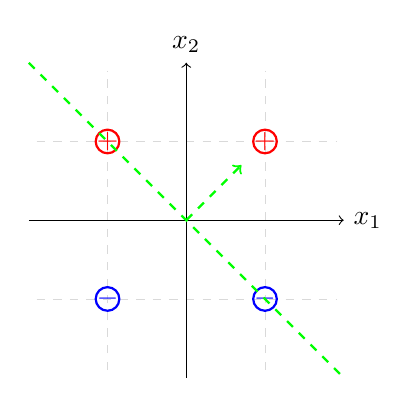
\begin{tikzpicture}
\draw[help lines, color=gray!30, dashed] (-1.9,-1.9) grid (1.9,1.9);
\draw[->] (-2,0)--(2,0) node[right]{$x_1$};
\draw[->] (0,-2)--(0,2) node[above]{$x_2$};
\draw [red, thick] (1,1) circle (.15cm) node[]{$+$};
\draw [red, thick] (-1,1) circle (.15cm) node[]{$+$};
\draw [blue, thick] (1,-1) circle (.15cm) node[]{$-$};
\draw [blue, thick] (-1,-1) circle (.15cm) node[]{$-$};
\draw [green, thick, dashed] (-2,2)--(2,-2);
\draw [->, green, thick, dashed] (0,0)--(.7,.7);
\end{tikzpicture}
\end{subfigure}
\begin{subfigure}[b]{0.3\textwidth}
\begin{tikzpicture}
\draw[help lines, color=gray!30, dashed] (-1.9,-1.9) grid (1.9,1.9);
\draw[->] (-2,0)--(2,0) node[right]{$x_1$};
\draw[->] (0,-2)--(0,2) node[above]{$x_2$};
\draw [red, thick] (1,1) circle (.15cm) node[]{$+$};
\draw [red, thick] (-1,1) circle (.15cm) node[]{$+$};
\draw [blue, thick] (1,-1) circle (.15cm) node[]{$-$};
\draw [blue, thick] (-1,-1) circle (.15cm) node[]{$-$};
\draw [green, thick, dashed] (-2,0)--(2,0);
\draw [->, green, thick, dashed] (0,0)--(0,1);
\end{tikzpicture}
\end{subfigure}

\caption{Example with $\frac{R^2}{\delta^2}=2$}
\label{fig:5}
\end{figure}

\subproblem{b}

\newpage
\problem{3}
\subproblem{a} The batch algorithm we are minimizing is \begin{equation*}
F(\mathbf{w_{i}}) = \sum_{j=1}^{n}\max(0, -y_{j}(\mathbf{w_{i}}\cdot \mathbf{x_{j}}))
\end{equation*}
The global minimum, 0, is achieved when all $n$ data points are classified correctly, i.e. $ y_{j}(\mathbf{w_{i}}\cdot x_{j}) \geq 0 $.
\par
So the gradient is $\nabla_{\mathbf{w}} F(\mathbf{w_{i}})= \sum_{j\in E}^{} y_{j}\mathbf{x_{j}} $ where $E$ is the set of all misclassified data points ( $y_{j}(\mathbf{w_{i}}\cdot x_{j}) \leq 0$). Note the that loop in line 5 uses line 7 to sum over the misclassified points, so this algorithm is computing the gradient at $\mathbf{w_{i}}$.
\par
\subproblem{b} Note the max element is only non-zero if $ 1 - y_{j}(\mathbf{w}\cdot \mathbf{x_{j}} \geq 0 \leftrightarrow 1 \geq y_{j}(\mathbf{w}\cdot \mathbf{x_{j}}$.  Let $E$ be that set of all data points such that this non-zero condition is satisfied.  Note this set includes misclassified points \textit{and} correctly classified points that are close to the hyperplane.  Taking the partial derivate of F wrt the $i^{th}$ element of $\mathbf{w}$ we have \begin{equation*}
F_{i}(\mathbf{w}) = w_{i} - C \sum_{j\in E} y_{j}x_{ji}
\end{equation*}
Stacking the partials, we can rewrite in the vector form $ \nabla_{\mathbf{w}} F(\mathbf{w}) = \mathbf{w} - C \sum_{j\in E} y_{j}\mathbf{x_{j}} $.
\par
The algorithm is updated as i) $\mathbf{w_{i}}$ where $i$ indicates the iteration; ii) $ 1 \geq y_{j}(\mathbf{w_{i}}\cdot \mathbf{x_{j}}$; iii) $\Delta\mathbf{w_{temp}} - Cy_{j}\mathbf{x_{j}} $
\par
\subproblem{c} The difference in the update condition is that algorithm 1 only uses points incorrectly classified and algorithm 2 uses misclassified points \textit{and} correctly classified points that are close to the hyperplane. So algorithm 2 includes more in examples in an update.  The order of the dataset will not affect the algorithms because they loop over all points when they update, not update one point at a time like the perceptron algorithm we discussed in lecture.
\par
\subproblem{d}
\subproblem{e}

\end{document}
